
%% bare_conf.tex
%% V1.4
%% 2012/12/27
%% by Michael Shell
%% See:
%% http://www.michaelshell.org/
%% for current contact information.
%%
%% This is a skeleton file demonstrating the use of IEEEtran.cls
%% (requires IEEEtran.cls version 1.8 or later) with an IEEE conference paper.
%%
%% Support sites:
%% http://www.michaelshell.org/tex/ieeetran/
%% http://www.ctan.org/tex-archive/macros/latex/contrib/IEEEtran/
%% and
%% http://www.ieee.org/

%%*************************************************************************
%% Legal Notice:
%% This code is offered as-is without any warranty either expressed or
%% implied; without even the implied warranty of MERCHANTABILITY or
%% FITNESS FOR A PARTICULAR PURPOSE! 
%% User assumes all risk.
%% In no event shall IEEE or any contributor to this code be liable for
%% any damages or losses, including, but not limited to, incidental,
%% consequential, or any other damages, resulting from the use or misuse
%% of any information contained here.
%%
%% All comments are the opinions of their respective authors and are not
%% necessarily endorsed by the IEEE.
%%
%% This work is distributed under the LaTeX Project Public License (LPPL)
%% ( http://www.latex-project.org/ ) version 1.3, and may be freely used,
%% distributed and modified. A copy of the LPPL, version 1.3, is included
%% in the base LaTeX documentation of all distributions of LaTeX released
%% 2003/12/01 or later.
%% Retain all contribution notices and credits.
%% ** Modified files should be clearly indicated as such, including  **
%% ** renaming them and changing author support contact information. **
%%
%% File list of work: IEEEtran.cls, IEEEtran_HOWTO.pdf, bare_adv.tex,
%%                    bare_conf.tex, bare_jrnl.tex, bare_jrnl_compsoc.tex,
%%                    bare_jrnl_transmag.tex
%%*************************************************************************

% *** Authors should verify (and, if needed, correct) their LaTeX system  ***
% *** with the testflow diagnostic prior to trusting their LaTeX platform ***
% *** with production work. IEEE's font choices can trigger bugs that do  ***
% *** not appear when using other class files.                            ***
% The testflow support page is at:
% http://www.michaelshell.org/tex/testflow/



% Note that the a4paper option is mainly intended so that authors in
% countries using A4 can easily print to A4 and see how their papers will
% look in print - the typesetting of the document will not typically be
% affected with changes in paper size (but the bottom and side margins will).
% Use the testflow package mentioned above to verify correct handling of
% both paper sizes by the user's LaTeX system.
%
% Also note that the "draftcls" or "draftclsnofoot", not "draft", option
% should be used if it is desired that the figures are to be displayed in
% draft mode.
%
\documentclass[conference]{IEEEtran}
% Add the compsoc option for Computer Society conferences.
%
% If IEEEtran.cls has not been installed into the LaTeX system files,
% manually specify the path to it like:
% \documentclass[conference]{../sty/IEEEtran}





% Some very useful LaTeX packages include:
% (uncomment the ones you want to load)


% *** MISC UTILITY PACKAGES ***
%
%\usepackage{ifpdf}
% Heiko Oberdiek's ifpdf.sty is very useful if you need conditional
% compilation based on whether the output is pdf or dvi.
% usage:
% \ifpdf
%   % pdf code
% \else
%   % dvi code
% \fi
% The latest version of ifpdf.sty can be obtained from:
% http://www.ctan.org/tex-archive/macros/latex/contrib/oberdiek/
% Also, note that IEEEtran.cls V1.7 and later provides a builtin
% \ifCLASSINFOpdf conditional that works the same way.
% When switching from latex to pdflatex and vice-versa, the compiler may
% have to be run twice to clear warning/error messages.






% *** CITATION PACKAGES ***
%
\usepackage{cite}
% cite.sty was written by Donald Arseneau
% V1.6 and later of IEEEtran pre-defines the format of the cite.sty package
% \cite{} output to follow that of IEEE. Loading the cite package will
% result in citation numbers being automatically sorted and properly
% "compressed/ranged". e.g., [1], [9], [2], [7], [5], [6] without using
% cite.sty will become [1], [2], [5]--[7], [9] using cite.sty. cite.sty's
% \cite will automatically add leading space, if needed. Use cite.sty's
% noadjust option (cite.sty V3.8 and later) if you want to turn this off
% such as if a citation ever needs to be enclosed in parenthesis.
% cite.sty is already installed on most LaTeX systems. Be sure and use
% version 4.0 (2003-05-27) and later if using .sty. cite.sty does
% not currently provide for hyperlinked citations.
% The latest version can be obtained at:
% http://www.ctan.org/tex-archive/macros/latex/contrib/cite/
% The documentation is contained in the cite.sty file itself.






% *** GRAPHICS RELATED PACKAGES ***
%
\ifCLASSINFOpdf
  \usepackage[pdftex]{graphicx}
  % declare the path(s) where your graphic files are
  % \graphicspath{{../pdf/}{../jpeg/}}
  % and their extensions so you won't have to specify these with
  % every instance of \includegraphics
  % \DeclareGraphicsExtensions{.pdf,.jpeg,.png}
\else
  % or other class option (dvipsone, dvipdf, if not using dvips). graphicx
  % will default to the driver specified in the system graphics.cfg if no
  % driver is specified.
  % \usepackage[dvips]{graphicx}
  % declare the path(s) where your graphic files are
  % \graphicspath{{../eps/}}
  % and their extensions so you won't have to specify these with
  % every instance of \includegraphics
  % \DeclareGraphicsExtensions{.eps}
\fi
% graphicx was written by David Carlisle and Sebastian Rahtz. It is
% required if you want graphics, photos, etc. graphicx.sty is already
% installed on most LaTeX systems. The latest version and documentation
% can be obtained at: 
% http://www.ctan.org/tex-archive/macros/latex/required/graphics/
% Another good source of documentation is "Using Imported Graphics in
% LaTeX2e" by Keith Reckdahl which can be found at:
% http://www.ctan.org/tex-archive/info/epslatex/
%
% latex, and pdflatex in dvi mode, support graphics in encapsulated
% postscript (.eps) format. pdflatex in pdf mode supports graphics
% in .pdf, .jpeg, .png and .mps (metapost) formats. Users should ensure
% that all non-photo figures use a vector format (.eps, .pdf, .mps) and
% not a bitmapped formats (.jpeg, .png). IEEE frowns on bitmapped formats
% which can result in "jaggedy"/blurry rendering of lines and letters as
% well as large increases in file sizes.
%
% You can find documentation about the pdfTeX application at:
% http://www.tug.org/applications/pdftex





% *** MATH PACKAGES ***
%
%\usepackage[cmex10]{amsmath}
% A popular package from the American Mathematical Society that provides
% many useful and powerful commands for dealing with mathematics. If using
% it, be sure to load this package with the cmex10 option to ensure that
% only type 1 fonts will utilized at all point sizes. Without this option,
% it is possible that some math symbols, particularly those within
% footnotes, will be rendered in bitmap form which will result in a
% document that can not be IEEE Xplore compliant!
%
% Also, note that the amsmath package sets \interdisplaylinepenalty to 10000
% thus preventing page breaks from occurring within multiline equations. Use:
%\interdisplaylinepenalty=2500
% after loading amsmath to restore such page breaks as IEEEtran.cls normally
% does. amsmath.sty is already installed on most LaTeX systems. The latest
% version and documentation can be obtained at:
% http://www.ctan.org/tex-archive/macros/latex/required/amslatex/math/





% *** SPECIALIZED LIST PACKAGES ***
%
%\usepackage{algorithmic}
% algorithmic.sty was written by Peter Williams and Rogerio Brito.
% This package provides an algorithmic environment fo describing algorithms.
% You can use the algorithmic environment in-text or within a figure
% environment to provide for a floating algorithm. Do NOT use the algorithm
% floating environment provided by algorithm.sty (by the same authors) or
% algorithm2e.sty (by Christophe Fiorio) as IEEE does not use dedicated
% algorithm float types and packages that provide these will not provide
% correct IEEE style captions. The latest version and documentation of
% algorithmic.sty can be obtained at:
% http://www.ctan.org/tex-archive/macros/latex/contrib/algorithms/
% There is also a support site at:
% http://algorithms.berlios.de/index.html
% Also of interest may be the (relatively newer and more customizable)
% algorithmicx.sty package by Szasz Janos:
% http://www.ctan.org/tex-archive/macros/latex/contrib/algorithmicx/




% *** ALIGNMENT PACKAGES ***
%
%\usepackage{array}
% Frank Mittelbach's and David Carlisle's array.sty patches and improves
% the standard LaTeX2e array and tabular environments to provide better
% appearance and additional user controls. As the default LaTeX2e table
% generation code is lacking to the point of almost being broken with
% respect to the quality of the end results, all users are strongly
% advised to use an enhanced (at the very least that provided by array.sty)
% set of table tools. array.sty is already installed on most systems. The
% latest version and documentation can be obtained at:
% http://www.ctan.org/tex-archive/macros/latex/required/tools/


% IEEEtran contains the IEEEeqnarray family of commands that can be used to
% generate multiline equations as well as matrices, tables, etc., of high
% quality.




% *** SUBFIGURE PACKAGES ***
%\ifCLASSOPTIONcompsoc
%  \usepackage[caption=false,font=normalsize,labelfont=sf,textfont=sf]{subfig}
%\else
%  \usepackage[caption=false,font=footnotesize]{subfig}
%\fi
% subfig.sty, written by Steven Douglas Cochran, is the modern replacement
% for subfigure.sty, the latter of which is no longer maintained and is
% incompatible with some LaTeX packages including fixltx2e. However,
% subfig.sty requires and automatically loads Axel Sommerfeldt's caption.sty
% which will override IEEEtran.cls' handling of captions and this will result
% in non-IEEE style figure/table captions. To prevent this problem, be sure
% and invoke subfig.sty's "caption=false" package option (available since
% subfig.sty version 1.3, 2005/06/28) as this is will preserve IEEEtran.cls
% handling of captions.
% Note that the Computer Society format requires a larger sans serif font
% than the serif footnote size font used in traditional IEEE formatting
% and thus the need to invoke different subfig.sty package options depending
% on whether compsoc mode has been enabled.
%
% The latest version and documentation of subfig.sty can be obtained at:
% http://www.ctan.org/tex-archive/macros/latex/contrib/subfig/




% *** FLOAT PACKAGES ***
%
%\usepackage{fixltx2e}
% fixltx2e, the successor to the earlier fix2col.sty, was written by
% Frank Mittelbach and David Carlisle. This package corrects a few problems
% in the LaTeX2e kernel, the most notable of which is that in current
% LaTeX2e releases, the ordering of single and double column floats is not
% guaranteed to be preserved. Thus, an unpatched LaTeX2e can allow a
% single column figure to be placed prior to an earlier double column
% figure. The latest version and documentation can be found at:
% http://www.ctan.org/tex-archive/macros/latex/base/


%\usepackage{stfloats}
% stfloats.sty was written by Sigitas Tolusis. This package gives LaTeX2e
% the ability to do double column floats at the bottom of the page as well
% as the top. (e.g., "\begin{figure*}[!b]" is not normally possible in
% LaTeX2e). It also provides a command:
%\fnbelowfloat
% to enable the placement of footnotes below bottom floats (the standard
% LaTeX2e kernel puts them above bottom floats). This is an invasive package
% which rewrites many portions of the LaTeX2e float routines. It may not work
% with other packages that modify the LaTeX2e float routines. The latest
% version and documentation can be obtained at:
% http://www.ctan.org/tex-archive/macros/latex/contrib/sttools/
% Do not use the stfloats baselinefloat ability as IEEE does not allow
% \baselineskip to stretch. Authors submitting work to the IEEE should note
% that IEEE rarely uses double column equations and that authors should try
% to avoid such use. Do not be tempted to use the cuted.sty or midfloat.sty
% packages (also by Sigitas Tolusis) as IEEE does not format its papers in
% such ways.
% Do not attempt to use stfloats with fixltx2e as they are incompatible.
% Instead, use Morten Hogholm'a dblfloatfix which combines the features
% of both fixltx2e and stfloats:
%
% \usepackage{dblfloatfix}
% The latest version can be found at:
% http://www.ctan.org/tex-archive/macros/latex/contrib/dblfloatfix/




% *** PDF, URL AND HYPERLINK PACKAGES ***
%
%\usepackage{url}
% url.sty was written by Donald Arseneau. It provides better support for
% handling and breaking URLs. url.sty is already installed on most LaTeX
% systems. The latest version and documentation can be obtained at:
% http://www.ctan.org/tex-archive/macros/latex/contrib/url/
% Basically, \url{my_url_here}.




% *** Do not adjust lengths that control margins, column widths, etc. ***
% *** Do not use packages that alter fonts (such as pslatex).         ***
% There should be no need to do such things with IEEEtran.cls V1.6 and later.
% (Unless specifically asked to do so by the journal or conference you plan
% to submit to, of course. )

\usepackage{hyperref}
\usepackage{listings}    
% correct bad hyphenation here
\hyphenation{op-tical net-works semi-conduc-tor}


\begin{document}
\lstset{
  frame=single,
  language=C,
  basicstyle=\small,
}

\makeatletter
\def\lst@makecaption{%
  \def\@captype{table}%
  \@makecaption
}
\makeatother
%
% paper title
% can use linebreaks \\ within to get better formatting as desired
% Do not put math or special symbols in the title.
\title{ABS Microservices and Ontology-Zotonic Integration for SPL Implementation in Information System}


% author names and affiliations
% use a multiple column layout for up to three different
% affiliations
\author{\IEEEauthorblockN{Andri Kurniawan}
\IEEEauthorblockA{Faculty of Computer Science\\
Universitas Indonesia\\
West Java, Indonesia\\
Email: andri.kurniawan31@ui.ac.id}
\and
\IEEEauthorblockN{Iis Afriyanti}
\IEEEauthorblockA{Faculty of Computer Science\\
Universitas Indonesia\\
West Java, Indonesia\\
Email: iisafriyanti@ui.ac.id}
\and
\IEEEauthorblockN{Ade Azurat}
\IEEEauthorblockA{Faculty of Computer Science\\
Universitas Indonesia\\
West Java, Indonesia\\
Email: ade@cs.ui.ac.id}}

% conference papers do not typically use \thanks and this command
% is locked out in conference mode. If really needed, such as for
% the acknowledgment of grants, issue a \IEEEoverridecommandlockouts
% after \documentclass

% for over three affiliations, or if they all won't fit within the width
% of the page, use this alternative format:
% 
%\author{\IEEEauthorblockN{Michael Shell\IEEEauthorrefmark{1},
%Homer Simpson\IEEEauthorrefmark{2},
%James Kirk\IEEEauthorrefmark{3}, 
%Montgomery Scott\IEEEauthorrefmark{3} and
%Eldon Tyrell\IEEEauthorrefmark{4}}
%\IEEEauthorblockA{\IEEEauthorrefmark{1}School of Electrical and Computer Engineering\\
%Georgia Institute of Technology,
%Atlanta, Georgia 30332--0250\\ Email: see http://www.michaelshell.org/contact.html}
%\IEEEauthorblockA{\IEEEauthorrefmark{2}Twentieth Century Fox, Springfield, USA\\
%Email: homer@thesimpsons.com}
%\IEEEauthorblockA{\IEEEauthorrefmark{3}Starfleet Academy, San Francisco, California 96678-2391\\
%Telephone: (800) 555--1212, Fax: (888) 555--1212}
%\IEEEauthorblockA{\IEEEauthorrefmark{4}Tyrell Inc., 123 Replicant Street, Los Angeles, California 90210--4321}}




% use for special paper notices
%\IEEEspecialpapernotice{(Invited Paper)}




% make the title area
\maketitle

% As a general rule, do not put math, special symbols or citations
% in the abstract
\begin{abstract}
Lorem Ipsum is simply dummy text of the printing and typesetting industry. Lorem Ipsum has been the industry's standard dummy text ever since the 1500s, when an unknown printer took a galley of type and scrambled it to make a type specimen book. It has survived not only five centuries, but also the leap into electronic typesetting, remaining essentially unchanged. It was popularised in the 1960s with the release of Letraset sheets containing Lorem Ipsum passages, and more recently with desktop publishing software like Aldus PageMaker including versions of Lorem Ipsum.
\end{abstract}

% no keywords




% For peer review papers, you can put extra information on the cover
% page as needed:
% \ifCLASSOPTIONpeerreview
% \begin{center} \bfseries EDICS Category: 3-BBND \end{center}
% \fi
%
% For peerreview papers, this IEEEtran command inserts a page break and
% creates the second title. It will be ignored for other modes.
\IEEEpeerreviewmaketitle

\section{Introduction} \label{introduction}
Software Product Line (SPL) gains a huge attention nowadays since it claims that using the paradigm can reduce the cost production, enhance the quality of product, and shorten time of distribution \cite{pohl:SPLE}. The fundamental key of SPL paradigm is feature model to capture the variabilities and commonalities of different product requirements for different stakeholders; some of previous product components can be used for other requirements. This paradigm has successfully adopted in industry area that several success stories can be found in Product Line Hall of Fame\footnote{http://splc.net/fame.html}. However, to the best of our knowledge, the automated SPL implementation in information system to have the system more adaptable is still inadequate. The main reason is that the feature model as a key part in SPL paradigm can not be executed as it is a model-oriented. Therefore, to realise automated SPL from requirement gathering to deployment phase, we need an executable model such as Abstract Behavioral Specification (ABS).

ABS becomes more promising to solve the problem in the SPL. It is a formal modelling language and executable for distributed object-oriented systems \cite{ABS}\cite{ABSTutorial}. The study of \cite{absmc} is to create a framework to accommodate requirement changes in SPL-based system by realizing ABS Microservices \cite{absmc}. The feature model is implemented into ABS Microservices and results a web service including the required business logic. The web service supports software development that meets the domain of feature model.

In addition, the previous study \cite{fmontology} presents the use of OWL ontology as a feature model representation to produce an application as part of SPL realization. By using such mechanism, it is possible to run inconsistency checking upon the feature model \cite{verify}. The feature model is mapped into \textit{classes} and \textit{object properties} of OWL ontology and can be transformed into Zotonic-based information system; a CMS which adopt pragmatic semantic web for its data model. The approach has already been adopted to automate a charity organization information system in \cite{bravyto}. However, the business logic for the system is still manually developed.

Since the web service produced by ABS Microservices provides business logic for the domain related with the feature model and can be retrieved via its web service, we can build an adaptor to integrate the web service resulted by ABS Microservices and the Zotonic-based system with ontology inside. Therefore, in this paper we attempt to develop the adaptor, in such a way the information system is semantically structured and the business logic is automatically developed and meets the requirement .

The remainder of this paper is structured as follows. Section \ref{relatedworks} describes some studies related with this paper. Section \ref{adaptor} explains the adaptor along with its implementation process. We also provide a case study of the adaptor for a charity organization in Section \ref{casestudy}. The last section concludes our work and explain the benefits of the adaptor. 

\section{Related Works} \label{relatedworks}

\begin{figure}[h]
\centering
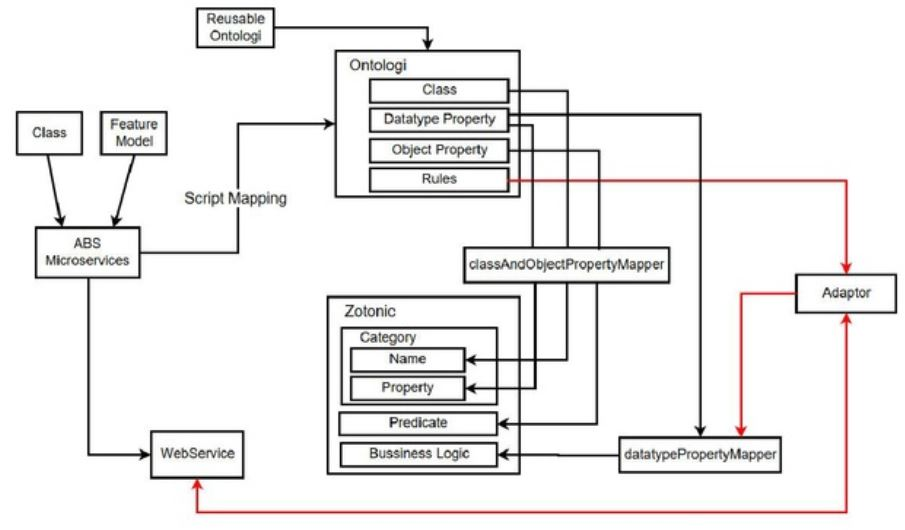
\includegraphics[width=3.5in]{overallsysdes}

\caption{Architectural Design SPL-based Information System}
\label{fig_sysdes}
\end{figure}

SPL becomes a promising paradigm in software development. In recent years, there has been increasing amount of literature on SPL realisation. Some attempts utilize Semantic Web in SPL process to gain more benefits of the paradigm. In \cite{fmontology} points out that ontology, as a main pillar of Semantic Web, accommodates application realisation production in SPL process with the help of Zotonic; a CMS with pragmatic semantic web for its data model. The study argues that within that it is possible to provide open and reasuable linked data of features.

The approach of study \cite{fmontology} is to translate every feature in the feature model into OWL classes. In addition, the relation between features is converted into OWL object property. The translation is implemented in Zotonic with BSMI charity organization as a case study (see Fig. \ref{fig_sysdes}). Each OWL class and object property are subsequently mapped into \textit{Category} and \textit{Predicate} of Zotonic system. The translation from OWL class and object properties runs automatically and results an information system. However, the system requires some business logic to be implemented, such as the total donation for charity organization system. In the previous study \cite{bravyto} the business logic of the system is implemented manually in Javascript. Although, business logic on one charity organizational with another may vary. 

On the other hand, the development of executable modelling language such as ABS \cite{ABS} also benefits the advancement of SPL. It provides a mechanism to implement the feature diagram into executable codes. A recent study by Afifun \cite{absmc} develops a microservices for ABS modelling language to support requirement changes and product variabilities in a product line. The microservices can also provide some business logic for the domain described in the feature model.

Thus, we attempt to implement an adaptor to integrate the ABS Microservices and Zotonic system that already included ontology of feature diagram as shown in Fig. \ref{fig_sysdes}. We employ Zotonic and the ontology as a representation of a feature model is mapped into Zotonic data model. Moreover, the adaptor employs the rules and the web service to provide business logic for the information system. By using the adaptor, the business logic required by the system will be retrieved from the web service, for example to calculate the total of donation for a certain charity program.

\section{Adaptor for ABS Microservices and Ontology-Zotonic Integration} \label{adaptor}
The adaptor is specifically built to call the web service produced by ABS Microservices. However, the adaptor needs a rules table which contains a list of methods along its endpoints in JSON format (see Fig \ref{fig_design}). When accessing a page that has business logic, the template engine generated by Zotonic which contains business logics will triggers the \textit{m\_abs} as illustrated in Fig. \ref{fig_design}. The m\_abs reads the rules table to identify the endpoint and total parameter in order to check whether the total parameter received is equalt to the web service requirement. Afterwards, the m\_abs will send the data to the web service to be processed. The full source code of this adaptor implementation can be found in \url{https://gitlab.com/andrikurniawan/adaptor-ontology-to-webservices}.

\begin{figure}[h]
\centering
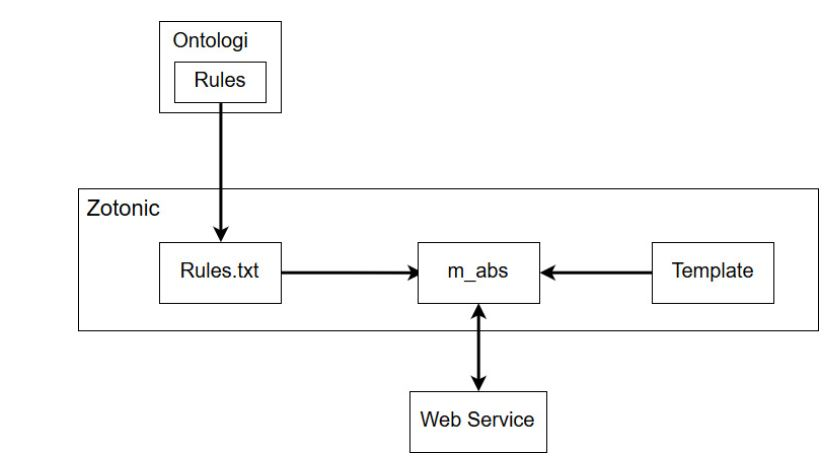
\includegraphics[width=3.5in]{adaptordesign}

\caption{Architecture Design of Adaptor}
\label{fig_design}
\end{figure}

%\begin{figure}[!t]
%\centering
%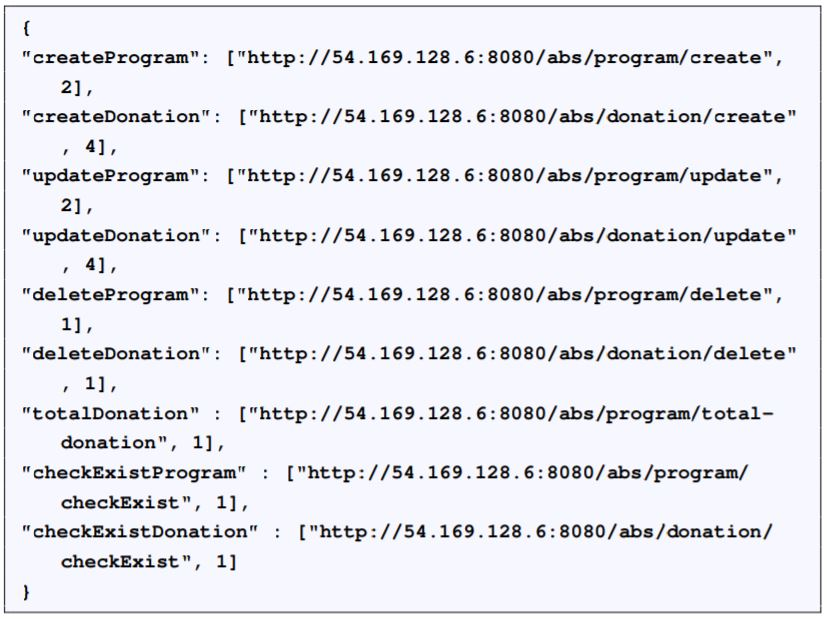
\includegraphics[width=3.5in]{Rules}
%
%\caption{Example of Rules}
%\label{fig_rules}
%\end{figure}

\subsection{Adaptor Interface}
The adaptor can be called by two options: \textit{template engine} and a \textit{model}. 

\subsubsection{Calling adaptor over template engine}
For this reason, we developed a new model inserted in Zotonic installation folder, we named it as m\_abs. Since it is a new model for Zotonic, we need to export the required built in models that is \texttt{m\_find\_value}, \texttt{m\_to\_list} and \texttt{m\_value}. We did not define \texttt{m\_to\_list} and \texttt{m\_value} since they will not be called when the adaptor is running.

However, we specify \texttt{m\_find\_value} to do pattern matching (see Listing \ref{mfindvalue}). When the template engine runs, it automatically generates some commands structured as \texttt{m.abs.functionName[{query param=value}]} and triggers the adaptor to run. For example \texttt{{{m.abs.totalDonation[{query id=id}]}}} means that it calls function \texttt{m\_abs} in the adaptor for \textit{totalDonation} method or \textit{key} and \texttt{{query id=id}} is the data which will be delivered to the web service. Both \textit{key} and \textit{data} are inputs for the parameters in \texttt{m\_find\_value} function.

\begin{lstlisting}[caption=Implementation of m\_find\_value function, label = mfindvalue]
m_find_value({query, Query}, #m{value=Q} =
 _, _Context) when is_list(Q) ->
 [Key] = Q,
 [Url, Param] = lookup_rules(Key),
 
 case validate_params(Param, Query) of
  
  false ->
   [{error, "Num of Params not same"}];
  
  true ->
   {DecodeJson} = fetch_data(binary_to_list
   (Url), jiffy:encode ({Query})),
   lager:info("ABS result : ~p", [DecodeJson]),
   proplists:get_value(<<"data">>, DecodeJson)

end;
\end{lstlisting}


\subsubsection{Calling adaptor by a \textit{model}}
The adaptor is also can be called from other models, such as \texttt{m\_src} model; one of Zotonic built in model. Regarding that requirement, we implemented a new function in the adaptor that is \texttt{call\_api\_controller} which can be accessed by other models. The function receives two paramaters: \textit{key} and \textit{data}. The \textit{key} indicates the method name in the web service and Data is to pass data to the web service. For example, \texttt{m\_abs:call\_api\_controller(deleteDonation, Json);} means that it calls function \texttt{call\_api\_controller} in the adaptor for \textit{deleteDonation} key and \texttt{Json} is the data which will be delivered to the web service. The benefit of calling the adaptor from another model is to be able to store the data from separate sites to the external centralized database.


\begin{lstlisting}[caption=Implementation of call\_api\_controller, label = callapicont]
 case proplists:get_value(<<"status">>, 
   DecodeJson) of 
   200 ->
     proplists:
       get_value(<<"data">>, DecodeJson),
   201 ->
     Message = proplists:
        get_value(<<"message">>, DecodeJson),
     lager:info("[ABS] status 201 ~p", 
       [binary_to_list(Message)]);
   400 ->
     Message = proplists:
        get_value(<<"message">>, DecodeJson),
     lager:error("[ABS] status 400 ~p", 
        [Message]);
        _Other ->
     lager:error("[ABS] status undefined ~p", 
        [_Other])
end
\end{lstlisting}

\subsection{Adaptor Implementation}
Aforementioned, the adaptor needs a table of rules. The rules is a JSON format and structured as in Listing \ref{rulestable}. The rules table must be located in root folder of Zotonic. 

\begin{lstlisting}[caption=Structure of Rules, label=rulestable]
{
 function name: [endpoint, total of parameter]
}
\end{lstlisting}

We also implemented \texttt{lookup\_rules} function to read the rules table then returns a list of endpoints along with its total of parameters with \textit{key} as an input. The function calls \texttt{read\_file} function which read the whole rules file. The adaptor also run \texttt{validate\_params} function which returns a boolean. If \textit{true} then the total parameter in rules table is same in the Query where query is data which will be delivered to the web service. If it returns true, the adaptor runs \texttt{fetch\_data} to request data from the web service. 

%\begin{lstlisting}[caption=Implementation of validate\_param, label=valparam]
%validate_params(Param, Query) ->
% case length(Query) == Param of
%  false ->
%   false;
%  true ->
%   true
%end.
%\end{lstlisting}

There are two parameters in \texttt{fetch\_data} function: \texttt{Url} and \texttt{Query}. The \texttt{Url} is the endpoint of web service and \texttt{Query} is parameter in JSON format. However, the function needs \texttt{post\_page\_body} to directly interact with the web service (see Listing \ref{postpagebody}).The function returns data in JSON format and decode with \texttt{jiffy:decode/1} 

\begin{lstlisting}[caption=Implementation of post\_page\_body function, label=postpagebody]
post_page_body(Url, Body) ->
 case httpc:request(post, {Url, [], 
    "application/json", Body},
    [], []) of
  {ok,{_, _, Response}} ->
    Response;
  Error ->
    {error, Error}
end.
\end{lstlisting} 

\begin{figure}[h]
\centering
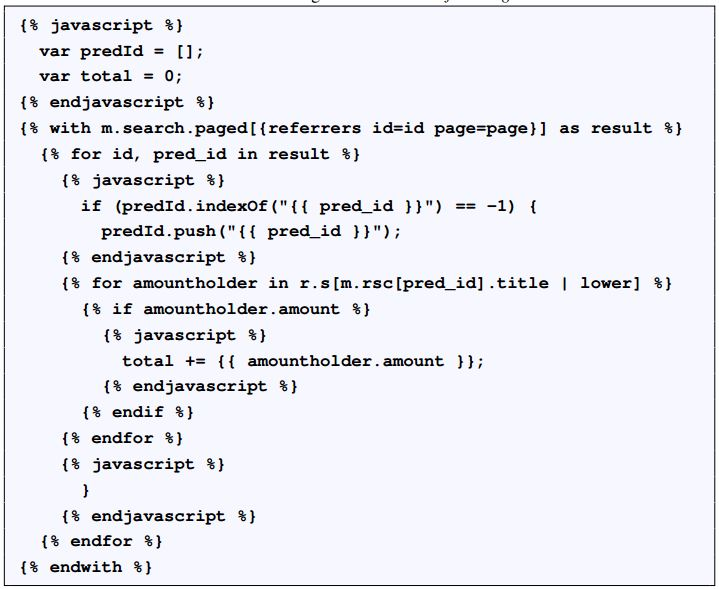
\includegraphics[width=3.5in]{totaldonationjs}

\caption{Total Donation function in Javascript}
\label{samplejs}
\end{figure}


\section{Case Study: BSMI Charity Organization} \label{casestudy}

%intro BSMI
BSMI (Bulan Sabit Merah Indonesia) is a charity organization that works to help others in Indonesia. To make it easier for the community to participate in providing assistance through BSMI, BSMI needs a website to facilitate their operations. In this paper, we employ BSMI as a case study to demonstrate the adaptor and its usage. 

BSMI has many features, but in this paper we focus on \textit{program}, \textit{donation}, \textit{target} and \textit{donor} features. Program feature provides charity activities undertaken by BSMI. Donation is a feature to store donations given by the communities for a charity program. Donor feature is to represent people who donate. Target feature are target of a program. The features have some business logic, for example, to calculate the total donation of a program. 

We adopt the ontology generated from the feature diagram in previous study \cite{bravyto} (see Fig. \ref{fig_ontaisco}). We added a table of rules to run the adaptor (see Fig. \ref{fig_rules}). For example, totalDonation is a rule to calculate the total of donation comes to the BSMI website, the endpoint of web service is "http://54.169.128.6:8080/abs/program/totaldonation", and the total parameter is 1. 

\begin{figure}[!t]
\centering
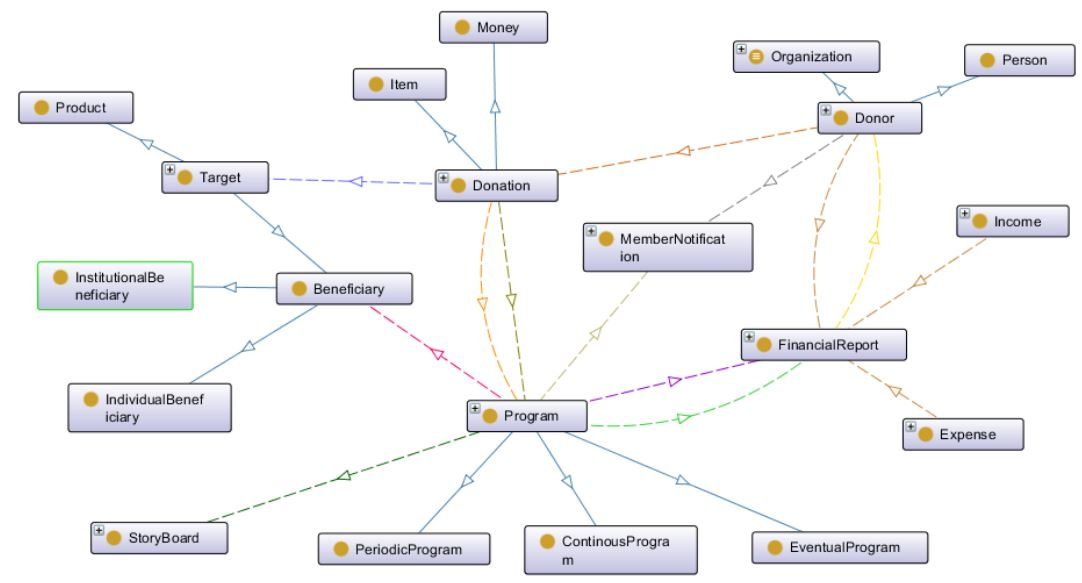
\includegraphics[width=3.5in]{aisco}

\caption{Ontology generated from the feature diagram of charity organization}
\label{fig_ontaisco}
\end{figure}

\begin{figure}[!t]
\centering
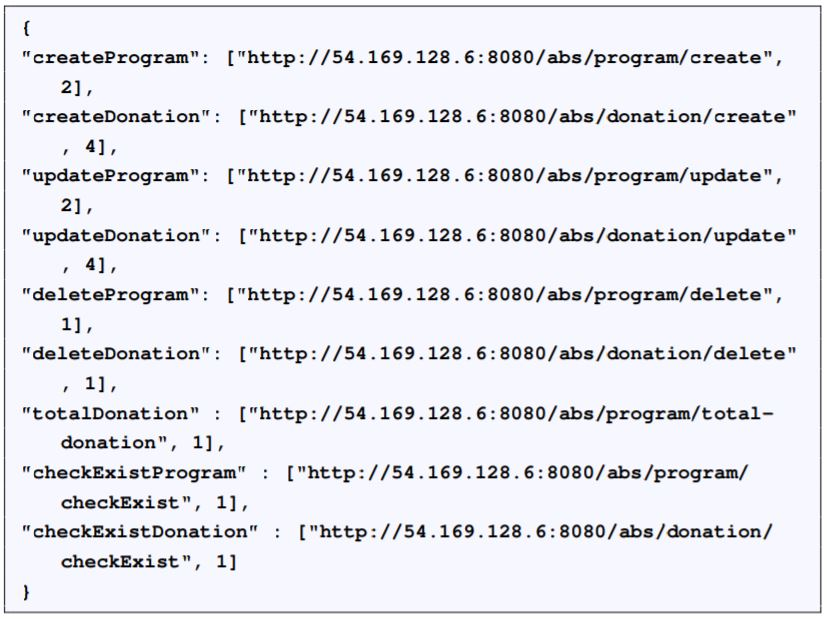
\includegraphics[width=3.5in]{Rules}

\caption{Example of Rules}
\label{fig_rules}
\end{figure}

When we open a page containing business logic, it will trigger the adaptor call. In this example, when opening a page with the category of program, total donation of that program will be automatically updated (see Fig. \ref{view_program}). If we create a new donation or delete a donation for this program, total donation in this program will be automatically updated.

\begin{figure}[h]
	\centering
	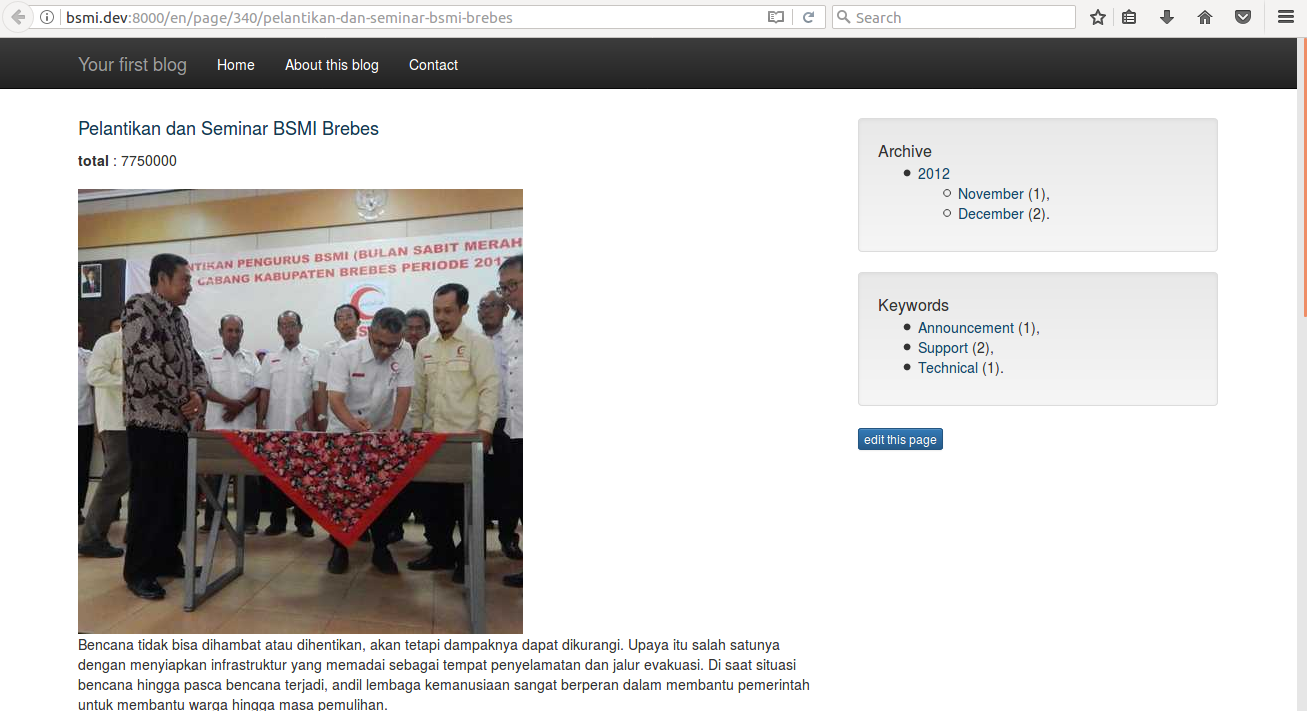
\includegraphics[width=3.5in]{19-viewProgram}
	
	\caption{View of "Pelantikan dan Seminar BSMI Brebes" program}
	\label{view_program}
\end{figure}

\\Andri please provide some example of calling adaptor by other models

\section{Conclusion} \label{conclusion}
In this paper we have presented an adaptor to integrate ABS Microservices and the ontology implemented in Zotonic-based information system. We explained the implementation process and show a case study in charity organization by adopting ontology from the previous study. The adaptor reads the \textit{rules} related with the ontology as a mapping table to call the web service. The adaptor can be called by the \textit{template engine} and other \textit{models}.

By utilising this adaptor, the business logic required by the information system can be generated automatically without manual development. In addition, the adaptor facilitates dynamic business logic that meets the requirement of the system. Therefore, we can generate several well-structured web pages with different business logics. Furthermore, we can deliver resources of the system into the web service by calling the adaptor from the models. From this scenario, it became apparent that an external global database can be produced since every information system can transfer its resources to the web service. 

\section*{Acknowledgment}
This work was fully supported by Reliable Software Engineering (RSE) Laboratory, Fasilkom UI and funded by Universitas Indonesia under Hibah PITTA no. 395/UN2.R3.1/HKP.05.00/2017



% trigger a \newpage just before the given reference
% number - used to balance the columns on the last page
% adjust value as needed - may need to be readjusted if
% the document is modified later
%\IEEEtriggeratref{8}
% The "triggered" command can be changed if desired:
%\IEEEtriggercmd{\enlargethispage{-5in}}

% references section

% can use a bibliography generated by BibTeX as a .bbl file
% BibTeX documentation can be easily obtained at:
% http://www.ctan.org/tex-archive/biblio/bibtex/contrib/doc/
% The IEEEtran BibTeX style support page is at:
% http://www.michaelshell.org/tex/ieeetran/bibtex/
%\bibliographystyle{IEEEtran}
% argument is your BibTeX string definitions and bibliography database(s)
%\bibliography{IEEEabrv,../bib/paper}
%
% <OR> manually copy in the resultant .bbl file
% set second argument of \begin to the number of references
% (used to reserve space for the reference number labels box)
\begin{thebibliography}{1}


\bibitem{pohl:SPLE}
K.~Pohl, G. B\"{o}ckle, and F. Van Der Linden, \textit{Software Product Line Engineering. Foundations, Principles, and Techniques}. Springer, 2005.

\bibitem{ABS}
E.~B.~Johnsen, R.~H\"{a}hnle, J.~Sch\"{a}fer, R.~Schlatte and M.~Steffen, \textit{ABS: A Core Language for Abstract Behavioral Specification}. Formal Methods for Components and Objects: 9th International Symposium, FMCO 2010, Graz, Austria, November 29 - December 1, 2010. Springer Berlin Heidelberg. Berlin, Heidelberg, 2012. 

\bibitem{ABSTutorial}
R.~H\"{a}hnle. \textit{The abstract behavioral specification language: A tutorial introduction}.
In Formal Methods for Components and Objects, pages 1–37. Springer, 2013.

\bibitem{fmontology}
I. Afriyanti, F.M. Falakh, A. Azurat and B. Takwa, \textit{Feature Model-to-Ontology for SPL Application Realisation}, submitted to The 18th International Conference on Product-Focused Software Process Improvement. URL: \url{https://arxiv.org/abs/1707.02511}

\bibitem{verify}
H. H. Wang, Y. F. Li, J. Sun, H. Zhang, and J. Pan, \textit{Verifying feature models using OWL}, Web Semantic, vol. 5, no. 2, pp. 117-129, 2007.


\bibitem{bravyto}
B. T. Pangukir, \textit{Pembentukan Otomatis Aplikasi Berbasis Web dengan Masukan Berupa Ontologi: Status Kasus Web BSMI}

\bibitem{absmc}
M. A. Naily, M. R. A. Setyautami, R. Muschevici, \textit{A Framework for Modelling Variable Microservices using the Abstract Behavioral Specification Language}, to appear in Microservices: Science and Engineering Workshop co-located with The 15th International Conference on Software Engineering and Formal Methods, Trento, Italy, September 4-8, 2017. 

\end{thebibliography}

% that's all folks
\end{document}


